\documentclass[12pt]{report}
\usepackage[utf8x]{inputenc}
\usepackage{graphicx}
\usepackage{gensymb}
\usepackage{algorithm}
\usepackage[noend]{algpseudocode}
\usepackage{algpseudocode}
\graphicspath{ {./images/} }
\usepackage{fancyhdr}
\newcommand{\R}{\mathbb{R}}

\title{ETERNITY : FUNCTIONS}								
\author{Juhi Birju Patel}						
\date{23 July 2022}

\makeatletter
\let\thetitle\@title
\let\theauthor\@author
\let\thedate\@date
\makeatother

\pagestyle{fancy}
\fancyhf{}
\rhead{\thetitle}
\cfoot{\thepage}

\begin{document}

\begin{titlepage}
	\centering
    \vspace*{0.5 cm}
\begin{center}    \textbf{\Large Concordia University}\\[2.0 cm]	\end{center}
	\textsc{\Large  SOEN 6011 - Software Engineering Process }\\[0.5 cm]
	\rule{\linewidth}{0.2 mm} \\[0.4 cm]
	{ \huge \textbf \thetitle}\\[0.2 cm]
	{ \huge \textbf{ Function 6 : B(x,y)}}
	\rule{\linewidth}{0.2 mm} \\[1.5 cm]

\begin{center}   {\Large Problem Solution 3}\\[2.0 cm]
\end{center}	
\begin{center}   {\Large \textbf{\theauthor}} \\[0.2 cm]
                 {\large Student ID : 40190446 }\\[0.2 cm]
                 {\large https://github.com/JuhiCodes/SOEN-6011-Course-Project}
\end{center}
	
\end{titlepage}

\tableofcontents
\pagebreak
\renewcommand{\thesection}{\arabic{section}}
\newpage
\section{Mindmap}
\begin{center}
   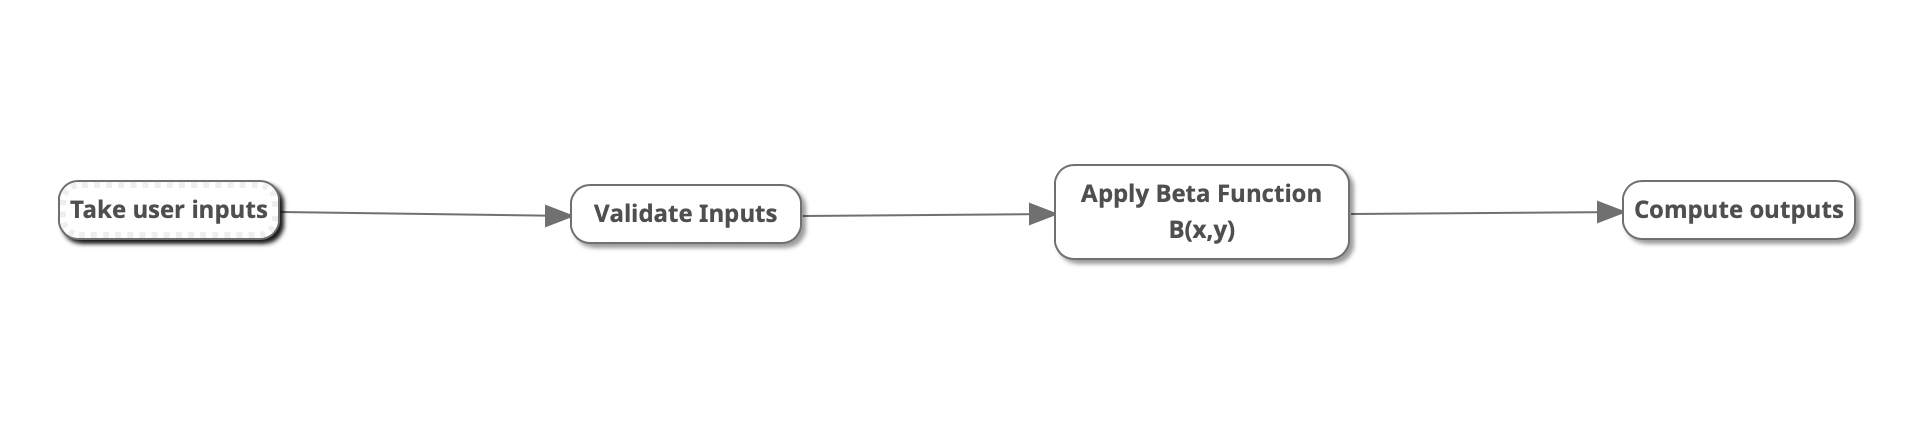
\includegraphics[scale=0.45]{images/mindmap.png}
    \end{center}
\section{Algorithms}
\subsection{Algorithm 1}
Stirling's approximation is used for calculating approximation of factorials. It is a good approximation which leads to accurate results even for small values of $n$. Stirling's approximation is defined as:\\
$$B(x,y)=\frac{\Gamma x \Gamma y}{\Gamma (x+y)}$$\\
\newline
$$\Gamma x = \sqrt{\frac{2 \pi}{x}}(\frac{x}{e})^x$$\\

\subsubsection{Technical reasons for selecting this algorithm}
\begin{itemize}
    \item It is easy to implement and provides with reliable approximation.
    \item It allows us to increase the domain of the function as it does not make use of any periodic functions.
\end{itemize}

\subsubsection{Advantages}
\begin{itemize}
\item The algorithm is easy to implement and reduces the complexity of the code.
\item The algorithm results in correct output for most of the inputs.
\item The algorithm works for all real positive numbers.
\item The algorithm provides an reliable estimation for the integral.
\end{itemize}

\subsubsection{Disadvantages}
\begin{itemize}
\item The algorithm is easy to implement but it is quite complex than other algorithms.
\item Debugging the code to spot the error is difficult hence time consuming.
\item The algorithm fails in providing accurate results.
\item The difference in the results for smaller input values id large.
\end{itemize}

\begin{algorithm}
\caption{Calculating Beta Function using Sterling's approximation}
\textbf{Input:}  $ (x,y) \in \mathbb{R}^{+}$\\
\textbf{Output:} $ Beta(x,y) $
\begin{algorithmic}[1]
\State $pi \leftarrow 3.141592653589793$
\State $e \leftarrow 2.718281828459045$

\Procedure {calculateBetaFunction}{$x, y, z$}
    \State $z \leftarrow x+y$
    \State $gammaX  \leftarrow \Call{CalculateGamma}{x}$
    \State $gammaY \leftarrow \Call{CalculateGamma}{y}$
    \State $gammaZ \leftarrow \Call{CalculateGamma}{z}$
    \State $beta \leftarrow \frac{gammaX *gammaY}{gammaZ}$
    \State \textbf{return} $beta$\Comment{Result}
    \EndProcedure
\Statex

\Procedure {CalculateGamma}{$num$}

        \State $num \leftarrow num - 1$
        \State $root \leftarrow 2 * pi * num$
        \State $sqRoot\leftarrow \Call {computeSquareRoot}{root}$
        \State $power \leftarrow \Call {computePower}{num,e}$
        \State \textbf{return} $(sqRoot) * (power)$\Comment{Result of gamma}
    \EndProcedure
\Statex
\Procedure {calculatePower}{$num1$,$num2$}
        \State $temp \leftarrow 1$
        \For $ i \leftarrow 1$ to $num2$
        \State $temp \leftarrow temp * num1$
        \EndFor
        \State \textbf{return} $temp$ \Comment{Result of power calculation}
    \EndProcedure
\Statex

\Procedure {calculateSquareRoot}{$ele$}
        \State $temp \leftarrow 0.0$
        \State $squareRoot \leftarrow ele / 2$
        \Do
        \State $temp \leftarrow squareRoot$
        \State $squareRoot \leftarrow (temp + (ele / temp)) / 2$
        \doWhile $((temp - squareRoot) != 0)$
        \State \textbf{return} $squareRoot $\Comment{return the square root}
    \EndProcedure
\Statex
\Statex
\State $beta \leftarrow \Call{calculateBetaFunction}{x,y}$

\end{algorithmic}
\end{algorithm}

\newpage
\subsection{Algorithm 2}
This algorithm calculates beta function using the gamma function in the factorial form for positive inputs.
\newline
$$B(x,y)=\frac{\Gamma x \Gamma y}{\Gamma (x+y)}$$\\
\newline
$$\Gamma x = (x-1)!$$\\
\subsubsection{Technical reasons for selecting this algorithm}
\begin{itemize}
    \item This algorithm is faster and easy to implement in any programming language.
    \item When the input to the function is integers, then this algorithm results in accurate results.
\end{itemize}

\subsubsection{Advantages}
\begin{itemize}
\item The algorithm is faster to compute the results.
\item The algorithm gives accurate results.
\item The algorithm is simple and easy to implement and debug.
\item The algorithm is more efficient to calculate beta function.
\end{itemize}

\subsubsection{Disadvantages}
\begin{itemize}
\item The algorithm works only for positive value inputs.
\item The algorithm fails when given negative inputs.
\item The algorithm doesn't work for integer inputs
\end{itemize}

\begin{algorithm}
\caption{Calculating Beta function using factorial function}

\textbf{Input:}  $ (x,y) \in \mathbb{R}^{+}$\\
\textbf{Output:} $ Beta(x,y)$
\begin{algorithmic}[1]

\Procedure {calculateGamma}{$num$}
    \State $num \leftarrow num-1$
    \State $gamma \leftarrow \Call{calculateFactorial}{num}$
    \State \textbf{return} $gamma$
    \EndProcedure
\Statex

\Procedure {calculateBetaFunction}{$x, y, z$}
    \State $z \leftarrow x+y$
    \State $gammaX  \leftarrow \Call{CalculateGamma}{x}$
    \State $gammaY \leftarrow \Call{CalculateGamma}{y}$
    \State $gammaZ \leftarrow \Call{CalculateGamma}{z}$
    \State $beta \leftarrow \frac{gammaX *gammaY}{gammaZ}$
    \State \textbf{return} $beta$\Comment{Result}
    \EndProcedure
\Statex

\Procedure {calculateFactorial}{$num$}
   
    \If{$num \leq 1 $}
    \State \textbf{return} $1$
    \Else
    \State \textbf{return} $num * calculateFactorial(num - 1)$
    \EndIf
    \EndProcedure
\Statex
\State $beta \leftarrow \Call{calculateBetaFunction}{x,y} $
\end{algorithmic}
\end{algorithm}

\newpage
\begin{thebibliography}{9}

\bibitem{wiki}
Wikipedia,
\\\texttt{https://en.wikipedia.org/wiki/Beta\_function}
\bibitem{stirling_wiki}
Stirlingwiki,
\\\texttt{https://en.wikipedia.org/wiki/Stirling\%27s\_approximation}
\bibitem{gamma}
Gamma,
\\\text{https://en.wikipedia.org/wiki/Gamma\_function}


\end{thebibliography}
\end{document}
